% !TeX root = main.tex

\chapter{Approximations}

Although the heuristic algorithms often produce excellent results, the biggest downside
is that they offer no guarantee from run to run. In contrast, an \textit{approximation algorithm}
promises that the answer is at most some fixed factor of the closest pair's distance.
More concretely, if we let $\delta$ be the distance of the closest pair, then
a \textit{$c$-approximate} closest pair is any pair whose distance is at most
$c \cdot \delta$, for some $c \geq 1$. People often write $c = 1 + \varepsilon$, where
$\varepsilon$ is thought of as the allowed error, and $\varepsilon = 0$ means we found the closest
pair. There are two kinds of approximation algorithms. \textit{Deterministic algorithms}
enforce the promise every run, whereas \textit{randomised algorithms}
guarantee that the promise holds with probability at least $p$
(which we call the \textit{confidence}).

\section{Deterministic Approximations}

\subsection{Chan's Shifted Z-order Curves}

\begin{figure}[ht]
    \centering
    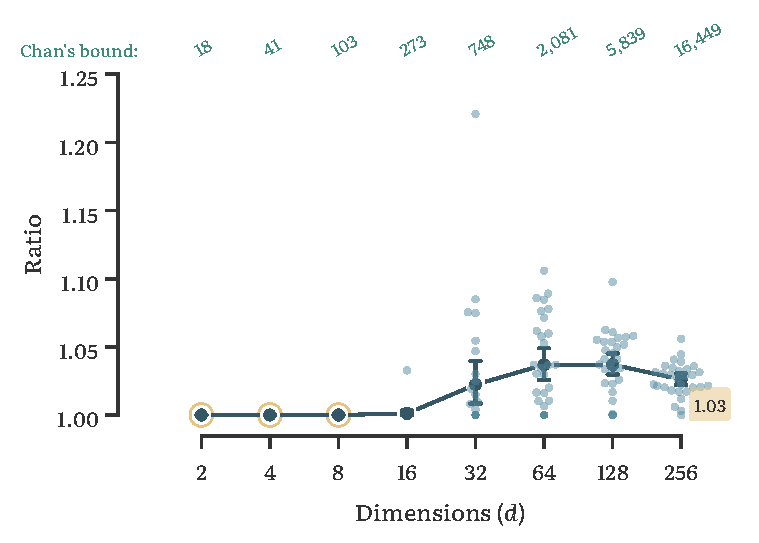
\includegraphics[scale=\figurescale]{diagrams/approximations_chan_bound.pdf}
    \caption{Ratio of Chan's shifted Z-order curves at $n = 10{,}000$. Chan's proven bound,
        $4d^{3/2} + 4d^{1/2} + 1$, is shown at the top for each $d$.
    }
    \label{fig:approximations_chan_bound}
\end{figure}

Recall that the Z-order curve provided a surprisingly good heuristic to put neighbouring
points close to each other in the sorted order. The main downside is that they could
end up on opposite sides of a grid boundary, so to compensate, we added random
shifts. It turns out that there is an alternative to random shifts. In 1998, Chan
showed that a fixed set of $d + 1$ shifts would suffice, where shift $j$ moves every
coordinate by $\sfrac{j}{d+1}$ of the grid's range ($j = 0, 1, \dots, d$)~\cite{chan1998}.
Under these fixed shifts, it may be proven that for any point, at any grid size, at
least one shift puts the point comfortably inside its grid cell. Thus, an adjacent pair
in one of the $d + 1$ shifts is within a constant factor of the closest pair, and this
constant depends only on $d$~\cite{chan2002}.

Instead of targeting the closest pair problem, Chan worked on the (arguably more popular)
nearest neighbour query. By checking the points just before and after the queried
point in each of the $d + 1$ shifts, the best point is within a factor of
$4d^{3/2} + 4d^{1/2} + 1$~\cite{chan1998}. Logically, if we iterate over all points and
call this nearest neighbour subroutine, one of these points must be part of the
closest pair, so the answer should be within the same factor. An implementation
detail is that Chan's lemma calls for even $d$, so for odd $d$, we'll use $d + 2$
shifts instead.

\subsection{The \texorpdfstring{$(1+\varepsilon)$}{(1 + epsilon)} \texorpdfstring{$k$}{k}-dimensional Tree}

Funnily enough, the $k$-dimensional tree has an approximate version as well.
The trick is to replace the ``budget'' in the heuristic version with a 
stopping rule from Arya et al.~\cite{arya1998}: stop once the nearest unvisited
region's lower bound, multiplied by $1 + \varepsilon$, reaches the best distance found so far.
The returned pair is always within $(1 + \varepsilon) \cdot \delta$.

\begin{figure}[ht]
    \centering
    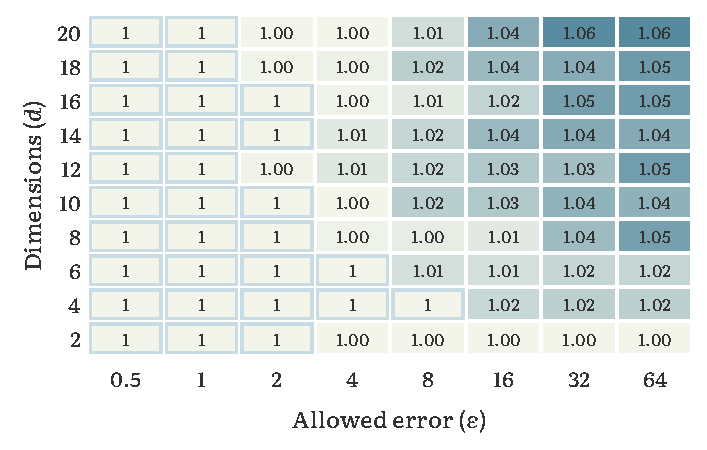
\includegraphics[scale=\figurescale]{diagrams/approximations_kd_tree_ratio.pdf}
    \caption{Mean ratio of the $(1 + \varepsilon)$ $k$-dimensional tree for each $d$ and $\varepsilon$, at
        $n = 10{,}000$. A cell marked 1 was exact in every trial.
    }
    \label{fig:approximations_kd_tree_ratio}
\end{figure}

Figures~\ref{fig:approximations_chan_bound} and~\ref{fig:approximations_kd_tree_ratio} unveil
the stark difference between what was promised and what was actually delivered, in a good way, of course.
For one, these approximations have to \textit{guarantee} that even in the worst case, we still hit
our $\varepsilon$ target, so they become overly strict in their pruning (especially in the case
of the $k$-dimensional tree). Even as we relax $\varepsilon$ to an unreasonable degree, the mean
ratios remain near one. Looking back, this should not be a total surprise, as the heuristics chapter
already demonstrated that in high dimensions, even random pairs give ratios of almost one. Nor does it
mean the approximation algorithms are useless, as having a provable bound offers us a way
to better appreciate the closest pair problem, rather than defaulting to empirical effectiveness.
